% Software Development for Mobile Devices
\documentclass[11pt,english,numbers=endperiod,parskip=half]{scrartcl}

\usepackage{color}
\usepackage{graphicx}
\usepackage{minted}
\usepackage{fancyhdr}
\usepackage{pdflscape}
\usepackage{listings}
\usepackage{pifont}

\newcommand{\cmark}{\ding{51}}

\pagestyle{fancy}

\rhead{Daniel Parker - 971328X}
\lhead{COS30017 - Software Development for Mobile Devices}

\title{Portfolio Report}
\subtitle{COS30017 - Software Development for Mobile Devices}
\author{Daniel Parker 971328X}

\date{\today}

\begin{document}
\maketitle
\thispagestyle{empty}

\section{Overview}

\section{Evidence}
\textit{\textbf{-} = in progress}
  \begin{table}[H]
    \begin{tabular}{|l|c|}
      \hline
      Assessment & Completed \\
      \hline
      Core Assignments (for Pass) & \cmark \\
      \hline
      Extension Tasks (for Credit) & \cmark \\
      \hline
      Custom Application (for Distinction) & \textbf{-} \\
      \hline
      Research Report (for HD) & \textbf{-} \\
      \hline
    \end{tabular}
  \end{table}
  Project brief has been submitted for custom application and I also intend on
  completing the HD research report as well.
\section{Reflection}
  \subsection{Concept Map}
    \begin{figure}[H]
    \centering{
      \fbox{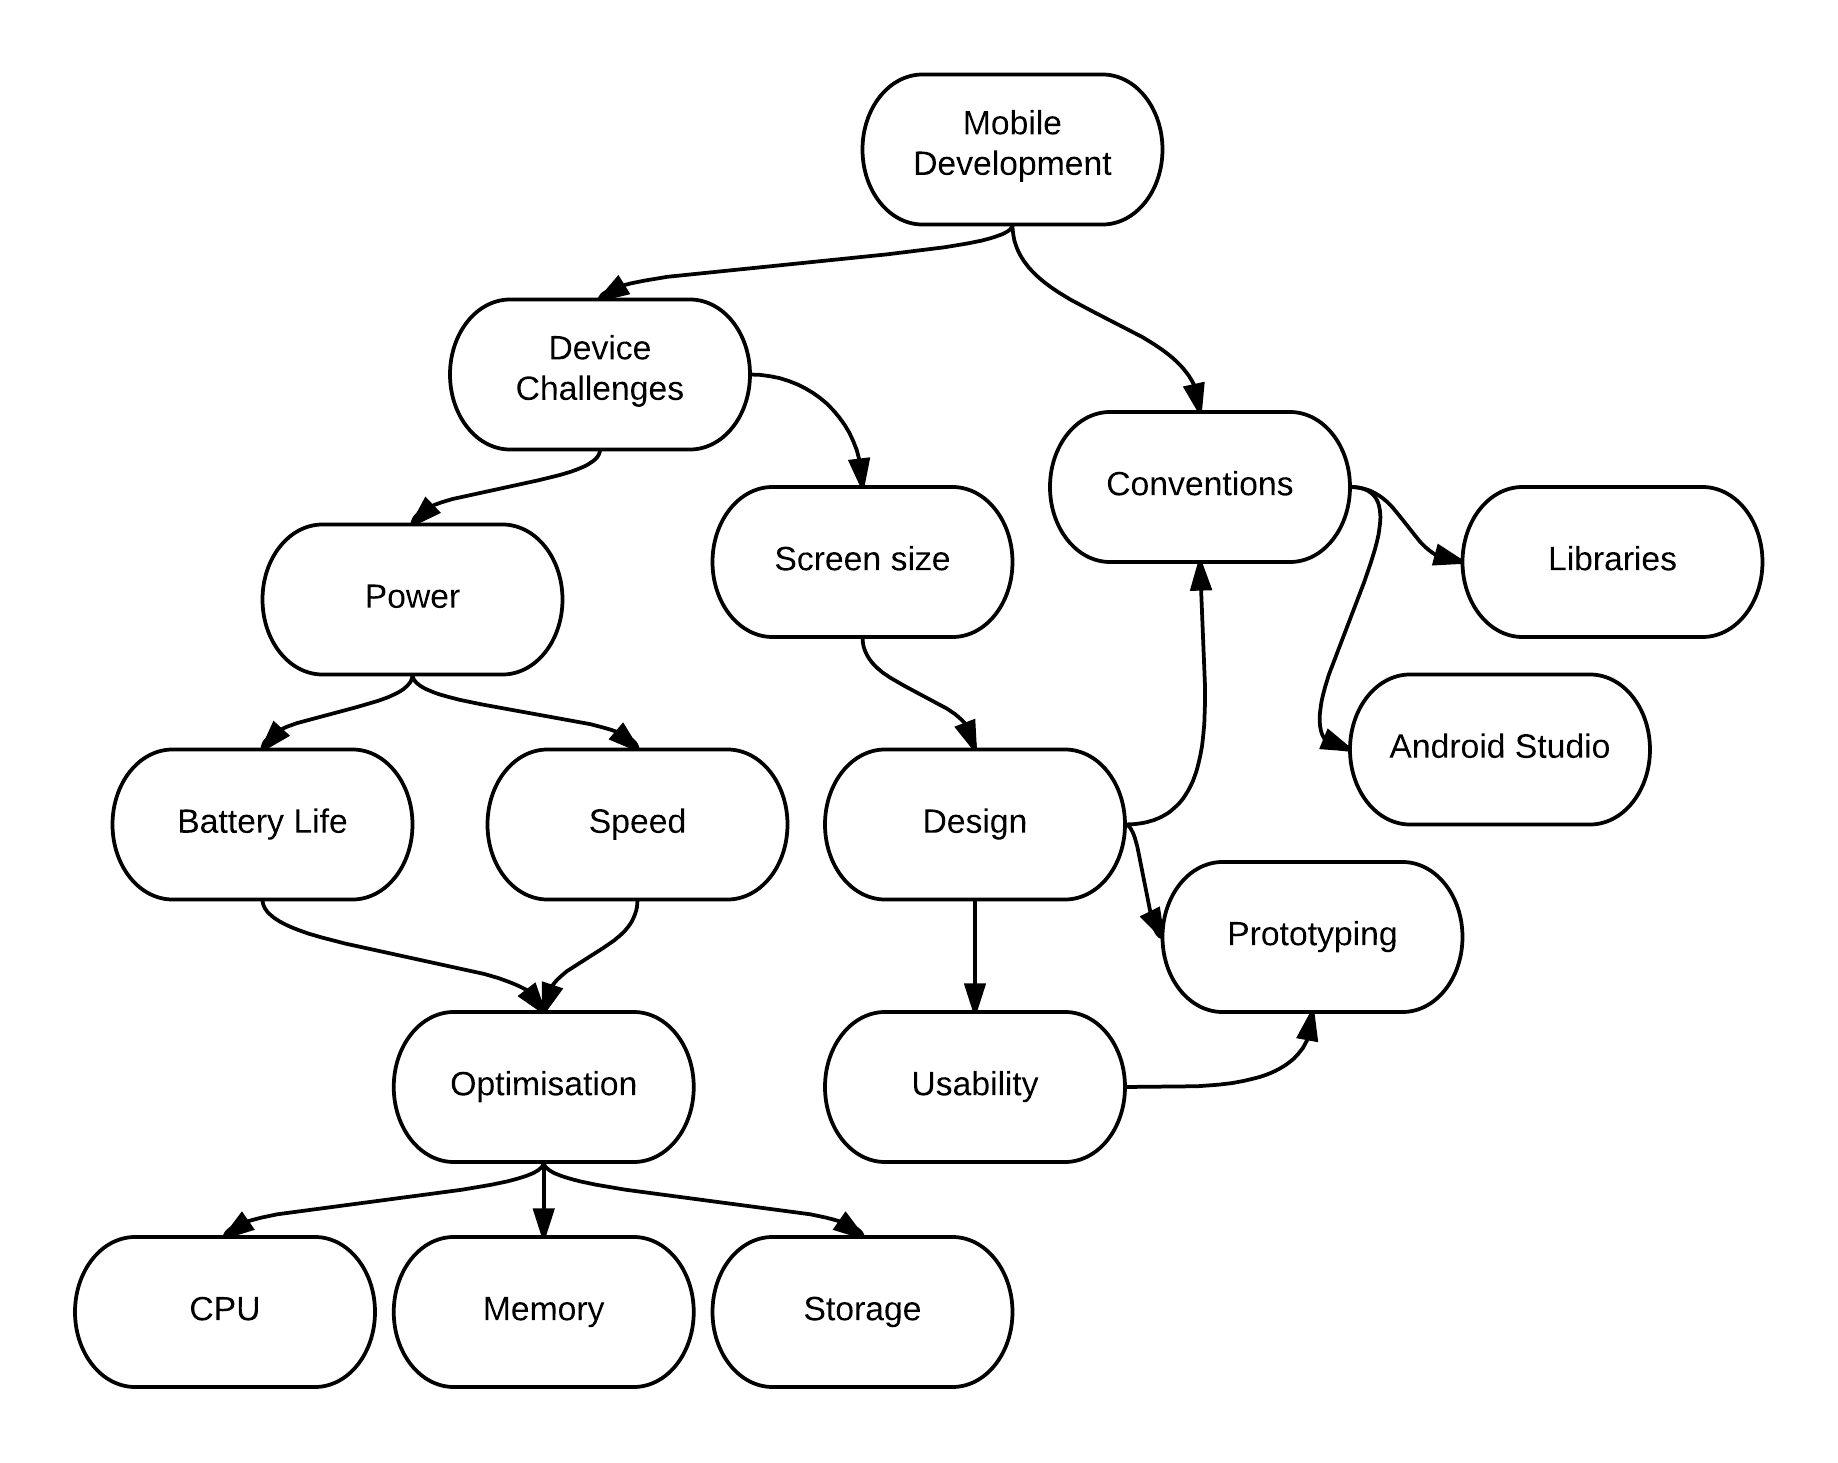
\includegraphics[width=\textwidth]{images/mind_map.png}}
    }\\
    \end{figure}
  \subsection{Mobile Application Development Process}
    The process to developing a mobile application is in a lot of ways a
    combination of web development and conventional desktop application development.
    From desktop application development comes the usual development methodologies
    such as agile, scrum etc., which are proven in providing a good and reliable
    framework for delivering applications. The web development processes that
    are also inherited by mobile development are those of iterative app design,
    user interface and usability testing, and then heavy design implementation.

    At a high level the resulting process for designing mobile applications is
    as follows:
    \begin{enumerate}
      \item{
        Ideation - Exploring the app's idea, what it will do, features etc.
      }
      \item{
        Exploration - User stories/scenarios, constraints, UI sketches and
        heuristic evaluation.
      }
      \item{
        Initial Clarification - Navigation flow, hi-fi prototype and usability
        test.
      }
      \item{
        Executable Prototype - Create prototype, validate the app.
      }
      \item{
        Iterative Development - Continue developing features, run usability
        tests and other validation methods to assist with refining.
      }
    \end{enumerate}
  \subsection{Analysis and Problem Solving Approaches}
    % SPEC:
    % Using an example illustrate how you can use the learning in the unit to
    % analyze a problem and/or solve it. You may also discuss the analysis or
    % problem solving approaches typically used in this area?

    Software engineering like other engineering disciplines requires that
    certain problems are solved. These problems are usually open-ended, vague,
    or have an inherent difficulty to them. The process of solving these problems
    usually involves some analysis of a problem, redefining of the problem to
    improve clarity and outline constraints, and then solving that problem using
    existing technical knowledge and research. This is an iterative process, and
    can take some time if the problem is complex or large.

    \textbf{Example:}
    \textit{`A chat program where users on mobile devices and also on a desktop
    browser webapp can send instant messages to each other without a long delay.'}

    \textbf{Analysis:}
    There are two key requirements in this sentence that will shift the way that
    the system is designed. The first is that the messages have to be sent without
    a long delay, and the second is that this must be true across mobiles and
    web browsers. A question that arises straight away is how long is a `long
    delay'? Also unknown is which web browsers need to be supported in this case
    and also what mobile OS and form factors need to be supported.

    \textbf{Refinement:}
    \textit{`A chat program where users of Android tablets (7 inch +) and desktop web
    browsers; Chrome, Safari and Internet Explorer 11 can communicate using
    instant messages where a message takes no longer than 5 seconds on average
    to reach the other user.`}

    \textbf{Constraints:}
    The redefined problem has enabled the extraction of concrete constraints:
    \begin{itemize}
      \item{
        The messages must reach their destination within 5 seconds.
      }
      \item{
        Must support Android tablets larger than 7 inches.
      }
      \item{
        Must support the browsers Chrome, Safari, and Internet Explorer 11.
      }
    \end{itemize}

    \textbf{Re-analysis:}
    Now that some of the ambiguities have been removed and initial constraints
    identified, the actual problem can be considered in more detail. A key issue
    that is already visible is that of having any message received no more than
    5 seconds after being sent. A naive solution to this is to have a persistent
    connection open between a server and all clients, however this introduces
    a lot of overhead to the server. In this case, due to there not being a
    minimum number of users required, it's arguable that this would be an easy
    solution.

    If there was a requirement for a minimum number of users then another
    solution is available which only took a small amount of online research to
    find. Socket.io is a project which allows for socket-like communcation in
    web browsers and other devices including Android. If socket.io didn't
    exist, then research would have to begin into how to build that kind of
    cross-platform and browser support.

    \textbf{Iterate...}

  \subsection{Comparison and Contextual Placement}
    Mobile development is different to developing command line processing
    software and is even different to developing websites, though it does have
    characteristics from both areas and is in may ways a combination of them.
    Mobile development requires the kind of design approaches long used in web
    development, but also commonly requires some module of complex underlying
    logic written in an OOP language. This makes mobile development quite different
    as a result and as such there are slight differences in the way that the
    development is practised.

    One aspect of Android development in particular that's accentuated heavily
    on is the concept of `Convention over Configuration', and this is apparent
    when using the newest Android integrated development environment, Android
    Studio. Every part of an Android application has it's place in the
    structure of the project, to the point where if it's not in that location,
    then the app may not compile correctly or at all. Anything to do with
    layout, design, dimensions, string constants and much more must be placed
    in their respective directories and xml files within the `res' directory,
    whereas any application logic needs to go in the `java' directory.

    Mobile development also requires that there is a greater emphasis on
    validating the UI decisions made. This is usually in the form of user tasks
    and usability tests both on prototypes and on a working executable of the
    app whilst it's in development. Design and usability of an app is paramount
    to it's success in the market of smartphone users, and if the app is either
    difficult to use or doesn't function exactly as required then it isn't
    likely to succeed. This is true of any application, however it seems to be
    a lot more important in mobile development, and much less likely to be
    excusable.

    The process of creating and designing mobile applications, both for Android
    and iOS has been somewhat simplified by the design guidelines and
    conventions that Google and Apple produce to assist developers in creating
    good apps for their platforms using their development kits.

  \subsection{Generalization}
    % SPEC:
    % Highlight ideas/techniques/principles that can be generalized and used in
    % other areas or for further learning (with a brief discussion to support the
    % claim). For instance, you can talk about how Convention over Configuration
    % can be used more generally.  Similarly, there are other concepts that you
    % can use more broadly.
    As was stated in an earlier section Android development makes heavy point of
    `Convention over Configuration'. This is something which is beneficial to
    development on that platform, due to the removal of many small decisions
    from the developer, increasing productivity and also the understandability
    of the codebase between developers, even those who aren't on the same team.
    Convention over Configuration would be hugely beneficial if it was more
    readily used in other areas of software development.

    Another aspect of Android development that could be used more generally in
    UI interface development is the pattern and abstraction of an Activity and
    Fragment. Android development requires that the Activity or Fragment classes
    are subclassed to create specific screens or screen components. That means
    that the subclass has the same lifecycle concepts as the superclass and
    any specific lifecycle events that need to be customised can just be
    overridden.

    The final generalization that would be beneficial is the Annotations library.
    Annotations allow the developer to quickly indicate some known functionality
    using an @ tag which is then compiled to its' known implementation. This is
    used for getting references to view objects, quickly register click handlers
    and various other functions which are considered to be boilerplate or
    heavily repeated code.

  \subsection{Challenges in Mobile Development}
    % SPEC:
    % Elaborate on aspects that your found challenging or different
    % (to expectations) and why?

  \subsection{Explorations}
    % SPEC:
    % Present information about areas that you have personally explored beyond the
    % expectations of the unit. Indicate areas where you plan to learn further on
    % your own and why?


\end{document}
